\documentclass[12pt]{article}\usepackage[]{graphicx}\usepackage[]{color}
%% maxwidth is the original width if it is less than linewidth
%% otherwise use linewidth (to make sure the graphics do not exceed the margin)
\makeatletter
\def\maxwidth{ %
  \ifdim\Gin@nat@width>\linewidth
    \linewidth
  \else
    \Gin@nat@width
  \fi
}
\makeatother

\definecolor{fgcolor}{rgb}{0.345, 0.345, 0.345}
\newcommand{\hlnum}[1]{\textcolor[rgb]{0.686,0.059,0.569}{#1}}%
\newcommand{\hlstr}[1]{\textcolor[rgb]{0.192,0.494,0.8}{#1}}%
\newcommand{\hlcom}[1]{\textcolor[rgb]{0.678,0.584,0.686}{\textit{#1}}}%
\newcommand{\hlopt}[1]{\textcolor[rgb]{0,0,0}{#1}}%
\newcommand{\hlstd}[1]{\textcolor[rgb]{0.345,0.345,0.345}{#1}}%
\newcommand{\hlkwa}[1]{\textcolor[rgb]{0.161,0.373,0.58}{\textbf{#1}}}%
\newcommand{\hlkwb}[1]{\textcolor[rgb]{0.69,0.353,0.396}{#1}}%
\newcommand{\hlkwc}[1]{\textcolor[rgb]{0.333,0.667,0.333}{#1}}%
\newcommand{\hlkwd}[1]{\textcolor[rgb]{0.737,0.353,0.396}{\textbf{#1}}}%

\usepackage{framed}
\makeatletter
\newenvironment{kframe}{%
 \def\at@end@of@kframe{}%
 \ifinner\ifhmode%
  \def\at@end@of@kframe{\end{minipage}}%
  \begin{minipage}{\columnwidth}%
 \fi\fi%
 \def\FrameCommand##1{\hskip\@totalleftmargin \hskip-\fboxsep
 \colorbox{shadecolor}{##1}\hskip-\fboxsep
     % There is no \\@totalrightmargin, so:
     \hskip-\linewidth \hskip-\@totalleftmargin \hskip\columnwidth}%
 \MakeFramed {\advance\hsize-\width
   \@totalleftmargin\z@ \linewidth\hsize
   \@setminipage}}%
 {\par\unskip\endMakeFramed%
 \at@end@of@kframe}
\makeatother

\definecolor{shadecolor}{rgb}{.97, .97, .97}
\definecolor{messagecolor}{rgb}{0, 0, 0}
\definecolor{warningcolor}{rgb}{1, 0, 1}
\definecolor{errorcolor}{rgb}{1, 0, 0}
\newenvironment{knitrout}{}{} % an empty environment to be redefined in TeX

\usepackage{alltt}
\usepackage{amsmath}
\usepackage{amssymb}
\usepackage{graphicx}
\usepackage{fullpage}
\usepackage{setspace}
\usepackage{hyperref}
\usepackage{color}
\onehalfspacing
\IfFileExists{upquote.sty}{\usepackage{upquote}}{}
\begin{document}

\title{Pol Sci 630: Problem Set 11 - Imputation of Missing Data, Regression Diagnostics, and Simulations - Solutions}

\author{Prepared by: Jan Vogler (\href{mailto:jan.vogler@duke.edu}{jan.vogler@duke.edu})}

\date{Grading Due Date: Friday, November 13th, 12.00 PM (Beginning of Lab)}
 
\maketitle



\textbf{\color{red} Insert your comments on the assignment that you are grading above the solution in bold and red text. For example write: "GRADER COMMENT: everything is correct! - 4/4 Points" Also briefly point out which, if any, problems were not solved correctly and what the mistake was.}

\bigskip

\textbf{Use the following scheme to assign points: For problems that were solved correctly in their entirety, assign the full point value of 4. For correctly solved bonus problems, add that value to the total score for a problem but do not go above 4 points per problem. If there are mistakes in any problem, subtract points according to the extent of the mistake. If you subtract points, explain why.}

\bigskip

\textbf{In order to make your text bold and red, you need to insert the following line at the beginning of the document:}

\begin{verbatim} \usepackage{color} \end{verbatim}

\textbf{and the following lines above the solution of the specific task:}

\begin{verbatim} \textbf{\color{red} GRADER COMMENT: everything is correct! - 4/4 Points} \end{verbatim}



\pagebreak

\section*{R Programming}

\subsection*{Problem 1}

\begin{knitrout}
\definecolor{shadecolor}{rgb}{0.969, 0.969, 0.969}\color{fgcolor}\begin{kframe}
\begin{alltt}
\hlkwd{setwd}\hlstd{(}\hlstr{"C:/Users/Jan/OneDrive/Documents/GitHub/ps630_lab/"}\hlstd{)}
\hlkwd{library}\hlstd{(foreign)}
\hlstd{LDC} \hlkwb{=} \hlkwd{read.dta}\hlstd{(}\hlstr{"LDC_IO_replication.dta"}\hlstd{)}

\hlstd{LDCs} \hlkwb{=} \hlkwd{subset}\hlstd{(LDC, ctylabel} \hlopt{==} \hlstr{"Brazil"} \hlopt{|} \hlstd{ctylabel} \hlopt{==} \hlstr{"Jamaica"} \hlopt{|} \hlstd{ctylabel} \hlopt{==}
    \hlstr{"Kuwait"} \hlopt{|} \hlstd{ctylabel} \hlopt{==} \hlstr{"HongKong"} \hlopt{|} \hlstd{ctylabel} \hlopt{==} \hlstr{"KyrgyzRepublic"}\hlstd{)}
\hlstd{keep} \hlkwb{=} \hlkwd{c}\hlstd{(}\hlstr{"ctylabel"}\hlstd{,} \hlstr{"date"}\hlstd{,} \hlstr{"newtar"}\hlstd{,} \hlstr{"fdignp"}\hlstd{,} \hlstr{"gdp_pc_95d"}\hlstd{,} \hlstr{"polityiv_update2"}\hlstd{)}
\hlstd{LDCs} \hlkwb{=} \hlstd{LDCs[, keep]}

\hlstd{lm1} \hlkwb{=} \hlkwd{lm}\hlstd{(fdignp} \hlopt{~} \hlstd{newtar} \hlopt{+} \hlstd{gdp_pc_95d} \hlopt{+} \hlstd{polityiv_update2,} \hlkwc{data} \hlstd{= LDCs)}
\hlkwd{summary}\hlstd{(lm1)}
\end{alltt}
\begin{verbatim}
## 
## Call:
## lm(formula = fdignp ~ newtar + gdp_pc_95d + polityiv_update2, 
##     data = LDCs)
## 
## Residuals:
##     Min      1Q  Median      3Q     Max 
## -2.9792 -1.0033 -0.1529  0.8006  4.9776 
## 
## Coefficients:
##                    Estimate Std. Error t value Pr(>|t|)   
## (Intercept)       4.9768361  1.6501106   3.016  0.00566 **
## newtar           -0.0710902  0.0312451  -2.275  0.03137 * 
## gdp_pc_95d       -0.0002303  0.0003059  -0.753  0.45824   
## polityiv_update2 -0.1065855  0.1017928  -1.047  0.30470   
## ---
## Signif. codes:  0 '***' 0.001 '**' 0.01 '*' 0.05 '.' 0.1 ' ' 1
## 
## Residual standard error: 1.812 on 26 degrees of freedom
##   (120 observations deleted due to missingness)
## Multiple R-squared:  0.2433,	Adjusted R-squared:  0.1559 
## F-statistic: 2.786 on 3 and 26 DF,  p-value: 0.0607
\end{verbatim}
\end{kframe}
\end{knitrout}



\begin{knitrout}
\definecolor{shadecolor}{rgb}{0.969, 0.969, 0.969}\color{fgcolor}\begin{kframe}
\begin{alltt}
\hlstd{a.out} \hlkwb{<-} \hlkwd{amelia}\hlstd{(LDCs,} \hlkwc{m} \hlstd{=} \hlnum{5}\hlstd{,} \hlkwc{ts} \hlstd{=} \hlstr{"date"}\hlstd{,} \hlkwc{cs} \hlstd{=} \hlstr{"ctylabel"}\hlstd{)}
\end{alltt}
\end{kframe}
\end{knitrout}

\begin{knitrout}
\definecolor{shadecolor}{rgb}{0.969, 0.969, 0.969}\color{fgcolor}\begin{kframe}
\begin{alltt}
\hlstd{lm2} \hlkwb{<-} \hlkwd{zelig}\hlstd{(fdignp} \hlopt{~} \hlstd{newtar} \hlopt{+} \hlstd{gdp_pc_95d} \hlopt{+} \hlstd{polityiv_update2,} \hlkwc{data} \hlstd{= a.out}\hlopt{$}\hlstd{imputations,}
    \hlkwc{model} \hlstd{=} \hlstr{"ls"}\hlstd{)}
\end{alltt}
\begin{verbatim}
## 
## 
##  How to cite this model in Zelig:
##   Kosuke Imai, Gary King, and Olivia Lau. 2015.
##   "ls: Least Squares Regression for Continuous Dependent Variables"
##   in Kosuke Imai, Gary King, and Olivia Lau, "Zelig: Everyone's Statistical Software,"
##   http://gking.harvard.edu/zelig
## 
\end{verbatim}
\begin{alltt}
\hlkwd{summary}\hlstd{(lm2)}
\end{alltt}
\begin{verbatim}
## 
##   Model: ls
##   Number of multiply imputed data sets: 5 
## 
## Combined results:
## 
## Call:
## lm(formula = formula, weights = weights, model = F, data = data)
## 
## Coefficients:
##                          Value   Std. Error     t-stat      p-value
## (Intercept)       4.7825511224 0.9280951222  5.1530829 0.0001891294
## newtar           -0.0692846804 0.0263073710 -2.6336604 0.0280189979
## gdp_pc_95d       -0.0003673317 0.0001984485 -1.8510179 0.1298043418
## polityiv_update2 -0.0139006929 0.0502203761 -0.2767939 0.7852298382
## 
## For combined results from datasets i to j, use summary(x, subset = i:j).
## For separate results, use print(summary(x), subset = i:j).
\end{verbatim}
\end{kframe}
\end{knitrout}

The results that every student will get can differ significantly. However, it is most likely that the second regression will yield different results than the first one.

Are these results from the first or the second regression more accurate (i.e. closer to the truth)? This is impossible to tell. Although multiple imputation potentially is a powerful tool in the sense that it allows us to make inferences about missing data points,these guesses have some uncertainty attached and we can never be fully certain about their accuracy.

Before we ran any regression we had a fairly small number of observations and many missing values for several of our variables. Does this mean that the imputation of data has improved our results? Considering that the imputation itself is also a process of statistical inference that relies on our data and considering that imputation is more precise the more data we have, the results of our imputation here are questionable in their accuracy.

It could be the case that the results from the second regression are more accurate than from the first one. The reverse could also be true. In short, we cannot say with certainty which of the two is better. Given that observations were missing in a systematic fashion, we should not have too much confidence in the results.

For grader: If you grade another students homework, then assign full points only if the student arrives at the conclusion that we cannot be certain which results are closer to the truth.



\subsection*{Problem 2}

\begin{knitrout}
\definecolor{shadecolor}{rgb}{0.969, 0.969, 0.969}\color{fgcolor}\begin{kframe}
\begin{alltt}
\hlstd{lm3} \hlkwb{=} \hlkwd{lm}\hlstd{(fdignp} \hlopt{~} \hlstd{l1polity} \hlopt{+} \hlstd{l1gdp_pc} \hlopt{+} \hlstd{l1lnpop,} \hlkwc{data} \hlstd{= LDC)}
\hlkwd{summary}\hlstd{(lm3)}
\end{alltt}
\begin{verbatim}
## 
## Call:
## lm(formula = fdignp ~ l1polity + l1gdp_pc + l1lnpop, data = LDC)
## 
## Residuals:
##     Min      1Q  Median      3Q     Max 
## -29.260  -1.389  -0.716   0.276 181.953 
## 
## Coefficients:
##               Estimate Std. Error t value Pr(>|t|)    
## (Intercept)  7.999e+00  1.131e+00   7.074 1.97e-12 ***
## l1polity     5.425e-02  1.617e-02   3.354 0.000808 ***
## l1gdp_pc     1.541e-05  7.461e-05   0.207 0.836337    
## l1lnpop     -3.972e-01  7.045e-02  -5.638 1.93e-08 ***
## ---
## Signif. codes:  0 '***' 0.001 '**' 0.01 '*' 0.05 '.' 0.1 ' ' 1
## 
## Residual standard error: 5.372 on 2392 degrees of freedom
##   (2974 observations deleted due to missingness)
## Multiple R-squared:  0.01755,	Adjusted R-squared:  0.01632 
## F-statistic: 14.24 on 3 and 2392 DF,  p-value: 3.354e-09
\end{verbatim}
\begin{alltt}
\hlkwd{library}\hlstd{(car)}
\end{alltt}


{\ttfamily\noindent\itshape\color{messagecolor}{\#\# \\\#\# Attaching package: 'car'\\\#\# \\\#\# The following object is masked from 'package:boot':\\\#\# \\\#\#\ \ \ \  logit}}\begin{alltt}
\hlkwd{crPlots}\hlstd{(lm3)}
\end{alltt}
\end{kframe}
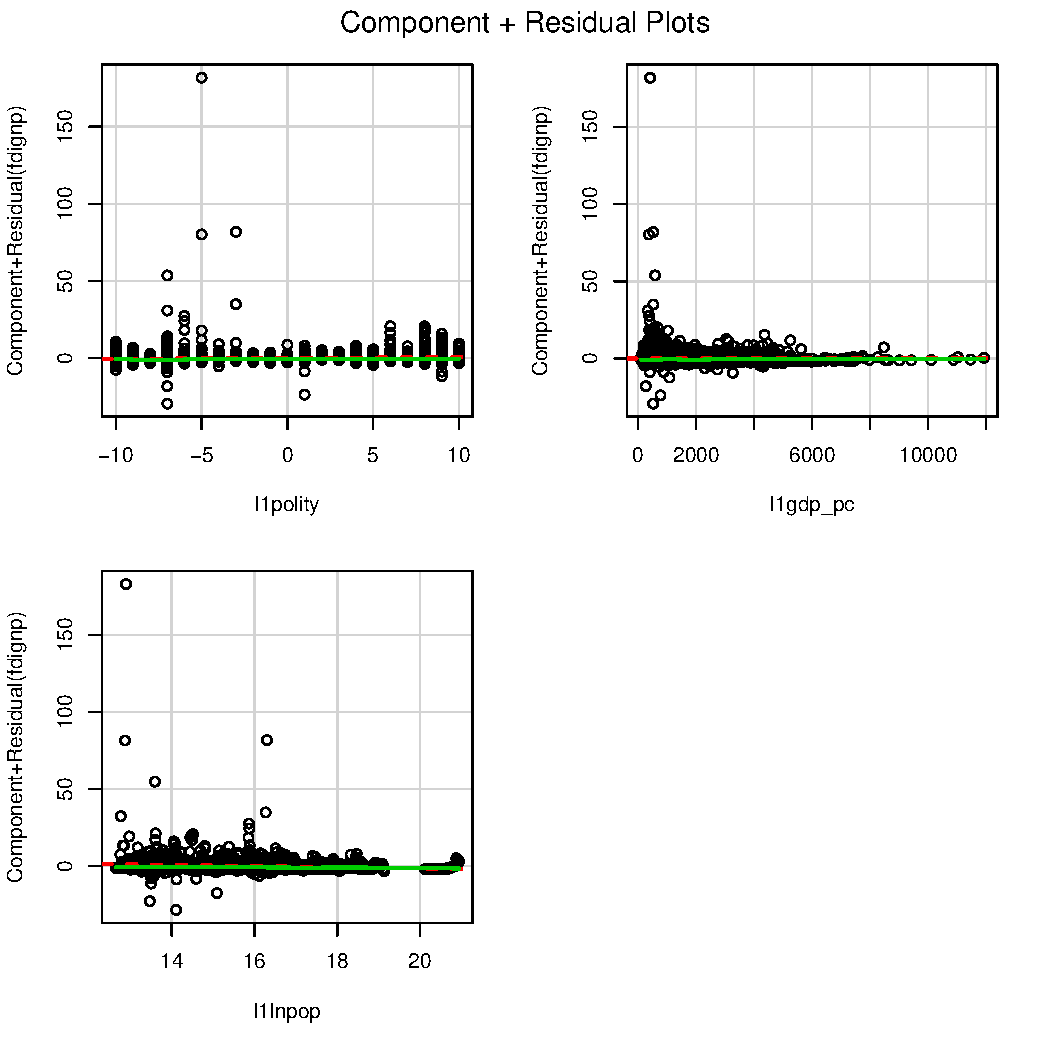
\includegraphics[width=\maxwidth]{figure/unnamed-chunk-5-1} 

\end{knitrout}

The component plus residual plots do not indicate any non-linear relationships for any of the variables utilized. There is a small amount of outliers for each of the three variables. However, those outliers do change the impression that there are generally linear trends.

\begin{knitrout}
\definecolor{shadecolor}{rgb}{0.969, 0.969, 0.969}\color{fgcolor}\begin{kframe}
\begin{alltt}
\hlkwd{library}\hlstd{(lmtest)}
\end{alltt}


{\ttfamily\noindent\itshape\color{messagecolor}{\#\# Loading required package: zoo\\\#\# \\\#\# Attaching package: 'zoo'\\\#\# \\\#\# The following objects are masked from 'package:base':\\\#\# \\\#\#\ \ \ \  as.Date, as.Date.numeric}}\begin{alltt}
\hlkwd{resettest}\hlstd{(lm3,} \hlkwc{power} \hlstd{=} \hlnum{2}\hlopt{:}\hlnum{3}\hlstd{,} \hlkwc{type} \hlstd{=} \hlkwd{c}\hlstd{(}\hlstr{"regressor"}\hlstd{),} \hlkwc{data} \hlstd{= LDC)}
\end{alltt}
\begin{verbatim}
## 
## 	RESET test
## 
## data:  lm3
## RESET = 5.5149, df1 = 6, df2 = 2386, p-value = 1.101e-05
\end{verbatim}
\end{kframe}
\end{knitrout}

The Ramsey RESET test yields a significant test result with $p < 0.001$, indicating that our model has not been specified correctly. We have to reject the null hypothesis that our model correctly captures the relationship. Therefore, including squared or cubic terms of our independent variables has the potential to improve the fit of our model.

Note that we should nonetheless be critical about including additional terms. The component plus residual plots have not revealed any strongly visible non-linear relationships. Like in other situations, there might be a trade off between overfitting the data and gaining higher R-squared values. (This second paragraph is not required from students.)



\subsection*{Problem 3}

\begin{knitrout}
\definecolor{shadecolor}{rgb}{0.969, 0.969, 0.969}\color{fgcolor}\begin{kframe}
\begin{alltt}
\hlstd{LDC} \hlkwb{=} \hlstd{LDC[}\hlkwd{with}\hlstd{(LDC,} \hlkwd{complete.cases}\hlstd{(newtar, l1polity, l1signed, l1office, l1gdp_pc,}
    \hlstd{l1lnpop, l1ecris2, l1bpc1)), ]}

\hlstd{lm4} \hlkwb{=} \hlkwd{lm}\hlstd{(newtar} \hlopt{~} \hlstd{l1polity} \hlopt{+} \hlstd{l1signed} \hlopt{+} \hlstd{l1office} \hlopt{+} \hlstd{l1gdp_pc} \hlopt{+} \hlstd{l1lnpop} \hlopt{+} \hlstd{l1ecris2} \hlopt{+}
    \hlstd{l1bpc1,} \hlkwc{data} \hlstd{= LDC)}
\hlkwd{summary}\hlstd{(lm4)}
\end{alltt}
\begin{verbatim}
## 
## Call:
## lm(formula = newtar ~ l1polity + l1signed + l1office + l1gdp_pc + 
##     l1lnpop + l1ecris2 + l1bpc1, data = LDC)
## 
## Residuals:
##     Min      1Q  Median      3Q     Max 
## -27.354  -8.404  -2.452   5.225  65.782 
## 
## Coefficients:
##               Estimate Std. Error t value Pr(>|t|)    
## (Intercept) -3.499e+01  5.958e+00  -5.873 6.68e-09 ***
## l1polity    -3.188e-01  8.649e-02  -3.686 0.000246 ***
## l1signed     1.195e+00  1.151e+00   1.038 0.299548    
## l1office    -1.870e-01  7.337e-02  -2.549 0.011014 *  
## l1gdp_pc    -1.237e-03  1.569e-04  -7.880 1.28e-14 ***
## l1lnpop      3.786e+00  3.376e-01  11.215  < 2e-16 ***
## l1ecris2    -8.246e+00  1.562e+00  -5.278 1.75e-07 ***
## l1bpc1       6.834e-01  1.016e+00   0.673 0.501424    
## ---
## Signif. codes:  0 '***' 0.001 '**' 0.01 '*' 0.05 '.' 0.1 ' ' 1
## 
## Residual standard error: 12.77 on 686 degrees of freedom
## Multiple R-squared:  0.3134,	Adjusted R-squared:  0.3064 
## F-statistic: 44.73 on 7 and 686 DF,  p-value: < 2.2e-16
\end{verbatim}
\begin{alltt}
\hlkwd{library}\hlstd{(arm)}
\end{alltt}


{\ttfamily\noindent\itshape\color{messagecolor}{\#\# Loading required package: Matrix\\\#\# Loading required package: lme4\\\#\# \\\#\# arm (Version 1.8-6, built: 2015-7-7)\\\#\# \\\#\# Working directory is C:/Users/Jan/OneDrive/Documents/GitHub/ps630\_lab/W11\\\#\# \\\#\# \\\#\# Attaching package: 'arm'\\\#\# \\\#\# The following object is masked from 'package:car':\\\#\# \\\#\#\ \ \ \  logit\\\#\# \\\#\# The following object is masked from 'package:Zelig':\\\#\# \\\#\#\ \ \ \  sim\\\#\# \\\#\# The following object is masked from 'package:boot':\\\#\# \\\#\#\ \ \ \  logit}}\begin{alltt}
\hlkwd{set.seed}\hlstd{(}\hlnum{2015}\hlstd{)}
\hlstd{model.sims} \hlkwb{=} \hlkwd{sim}\hlstd{(lm4,} \hlkwc{n.sims} \hlstd{=} \hlnum{1000}\hlstd{)}

\hlkwd{curve}\hlstd{(}\hlkwd{coef}\hlstd{(lm4)[}\hlnum{1}\hlstd{]} \hlopt{+} \hlkwd{coef}\hlstd{(lm4)[}\hlnum{2}\hlstd{]} \hlopt{*} \hlstd{x} \hlopt{+} \hlkwd{coef}\hlstd{(lm4)[}\hlnum{3}\hlstd{]} \hlopt{*} \hlkwd{mean}\hlstd{(LDC}\hlopt{$}\hlstd{l1signed,} \hlkwc{na.rm} \hlstd{= T)} \hlopt{+}
    \hlkwd{coef}\hlstd{(lm4)[}\hlnum{4}\hlstd{]} \hlopt{*} \hlkwd{mean}\hlstd{(LDC}\hlopt{$}\hlstd{l1office,} \hlkwc{na.rm} \hlstd{= T)} \hlopt{+} \hlkwd{coef}\hlstd{(lm4)[}\hlnum{5}\hlstd{]} \hlopt{*} \hlkwd{mean}\hlstd{(LDC}\hlopt{$}\hlstd{l1gdp_pc,}
    \hlkwc{na.rm} \hlstd{= T)} \hlopt{+} \hlkwd{coef}\hlstd{(lm4)[}\hlnum{6}\hlstd{]} \hlopt{*} \hlkwd{mean}\hlstd{(LDC}\hlopt{$}\hlstd{l1lnpop,} \hlkwc{na.rm} \hlstd{= T)} \hlopt{+} \hlkwd{coef}\hlstd{(lm4)[}\hlnum{7}\hlstd{]} \hlopt{*}
    \hlkwd{mean}\hlstd{(LDC}\hlopt{$}\hlstd{l1ecris2,} \hlkwc{na.rm} \hlstd{= T)} \hlopt{+} \hlkwd{coef}\hlstd{(lm4)[}\hlnum{8}\hlstd{]} \hlopt{*} \hlkwd{mean}\hlstd{(LDC}\hlopt{$}\hlstd{l1bpc1,} \hlkwc{na.rm} \hlstd{= T),}
    \hlkwc{from} \hlstd{=} \hlopt{-}\hlnum{10}\hlstd{,} \hlkwc{to} \hlstd{=} \hlnum{10}\hlstd{,} \hlkwc{ylim} \hlstd{=} \hlkwd{c}\hlstd{(}\hlopt{-}\hlnum{5}\hlstd{,} \hlnum{45}\hlstd{),} \hlkwc{xlab} \hlstd{=} \hlstr{"Polity IV Score (t-1)"}\hlstd{,} \hlkwc{ylab} \hlstd{=} \hlstr{"Tariff Level"}\hlstd{,}
    \hlkwc{main} \hlstd{=} \hlstr{"Tariff Level as Function of the Polity IV Score (t-1)"}\hlstd{,} \hlkwc{lwd} \hlstd{=} \hlnum{2}\hlstd{)}
\hlkwa{for} \hlstd{(i} \hlkwa{in} \hlnum{1}\hlopt{:}\hlnum{1000}\hlstd{) \{}
    \hlkwd{curve}\hlstd{(}\hlkwd{coef}\hlstd{(model.sims)[i,} \hlnum{1}\hlstd{]} \hlopt{+} \hlkwd{coef}\hlstd{(model.sims)[i,} \hlnum{2}\hlstd{]} \hlopt{*} \hlstd{x} \hlopt{+} \hlkwd{coef}\hlstd{(model.sims)[i,}
        \hlnum{3}\hlstd{]} \hlopt{*} \hlkwd{mean}\hlstd{(LDC}\hlopt{$}\hlstd{l1signed,} \hlkwc{na.rm} \hlstd{= T)} \hlopt{+} \hlkwd{coef}\hlstd{(model.sims)[i,} \hlnum{4}\hlstd{]} \hlopt{*} \hlkwd{mean}\hlstd{(LDC}\hlopt{$}\hlstd{l1office,}
        \hlkwc{na.rm} \hlstd{= T)} \hlopt{+} \hlkwd{coef}\hlstd{(model.sims)[i,} \hlnum{5}\hlstd{]} \hlopt{*} \hlkwd{mean}\hlstd{(LDC}\hlopt{$}\hlstd{l1gdp_pc,} \hlkwc{na.rm} \hlstd{= T)} \hlopt{+}
        \hlkwd{coef}\hlstd{(model.sims)[i,} \hlnum{6}\hlstd{]} \hlopt{*} \hlkwd{mean}\hlstd{(LDC}\hlopt{$}\hlstd{l1lnpop,} \hlkwc{na.rm} \hlstd{= T)} \hlopt{+} \hlkwd{coef}\hlstd{(model.sims)[i,}
        \hlnum{7}\hlstd{]} \hlopt{*} \hlkwd{mean}\hlstd{(LDC}\hlopt{$}\hlstd{l1ecris2,} \hlkwc{na.rm} \hlstd{= T)} \hlopt{+} \hlkwd{coef}\hlstd{(model.sims)[i,} \hlnum{8}\hlstd{]} \hlopt{*} \hlkwd{mean}\hlstd{(LDC}\hlopt{$}\hlstd{l1bpc1,}
        \hlkwc{na.rm} \hlstd{= T),} \hlkwc{add} \hlstd{=} \hlnum{TRUE}\hlstd{,} \hlkwc{col} \hlstd{=} \hlstr{"gray80"}\hlstd{)}
\hlstd{\}}
\hlkwd{curve}\hlstd{(}\hlkwd{coef}\hlstd{(lm4)[}\hlnum{1}\hlstd{]} \hlopt{+} \hlkwd{coef}\hlstd{(lm4)[}\hlnum{2}\hlstd{]} \hlopt{*} \hlstd{x} \hlopt{+} \hlkwd{coef}\hlstd{(lm4)[}\hlnum{3}\hlstd{]} \hlopt{*} \hlkwd{mean}\hlstd{(LDC}\hlopt{$}\hlstd{l1signed,} \hlkwc{na.rm} \hlstd{= T)} \hlopt{+}
    \hlkwd{coef}\hlstd{(lm4)[}\hlnum{4}\hlstd{]} \hlopt{*} \hlkwd{mean}\hlstd{(LDC}\hlopt{$}\hlstd{l1office,} \hlkwc{na.rm} \hlstd{= T)} \hlopt{+} \hlkwd{coef}\hlstd{(lm4)[}\hlnum{5}\hlstd{]} \hlopt{*} \hlkwd{mean}\hlstd{(LDC}\hlopt{$}\hlstd{l1gdp_pc,}
    \hlkwc{na.rm} \hlstd{= T)} \hlopt{+} \hlkwd{coef}\hlstd{(lm4)[}\hlnum{6}\hlstd{]} \hlopt{*} \hlkwd{mean}\hlstd{(LDC}\hlopt{$}\hlstd{l1lnpop,} \hlkwc{na.rm} \hlstd{= T)} \hlopt{+} \hlkwd{coef}\hlstd{(lm4)[}\hlnum{7}\hlstd{]} \hlopt{*}
    \hlkwd{mean}\hlstd{(LDC}\hlopt{$}\hlstd{l1ecris2,} \hlkwc{na.rm} \hlstd{= T)} \hlopt{+} \hlkwd{coef}\hlstd{(lm4)[}\hlnum{8}\hlstd{]} \hlopt{*} \hlkwd{mean}\hlstd{(LDC}\hlopt{$}\hlstd{l1bpc1,} \hlkwc{na.rm} \hlstd{= T),}
    \hlkwc{col} \hlstd{=} \hlstr{"black"}\hlstd{,} \hlkwc{lwd} \hlstd{=} \hlnum{2}\hlstd{,} \hlkwc{add} \hlstd{=} \hlnum{TRUE}\hlstd{)}
\end{alltt}
\end{kframe}
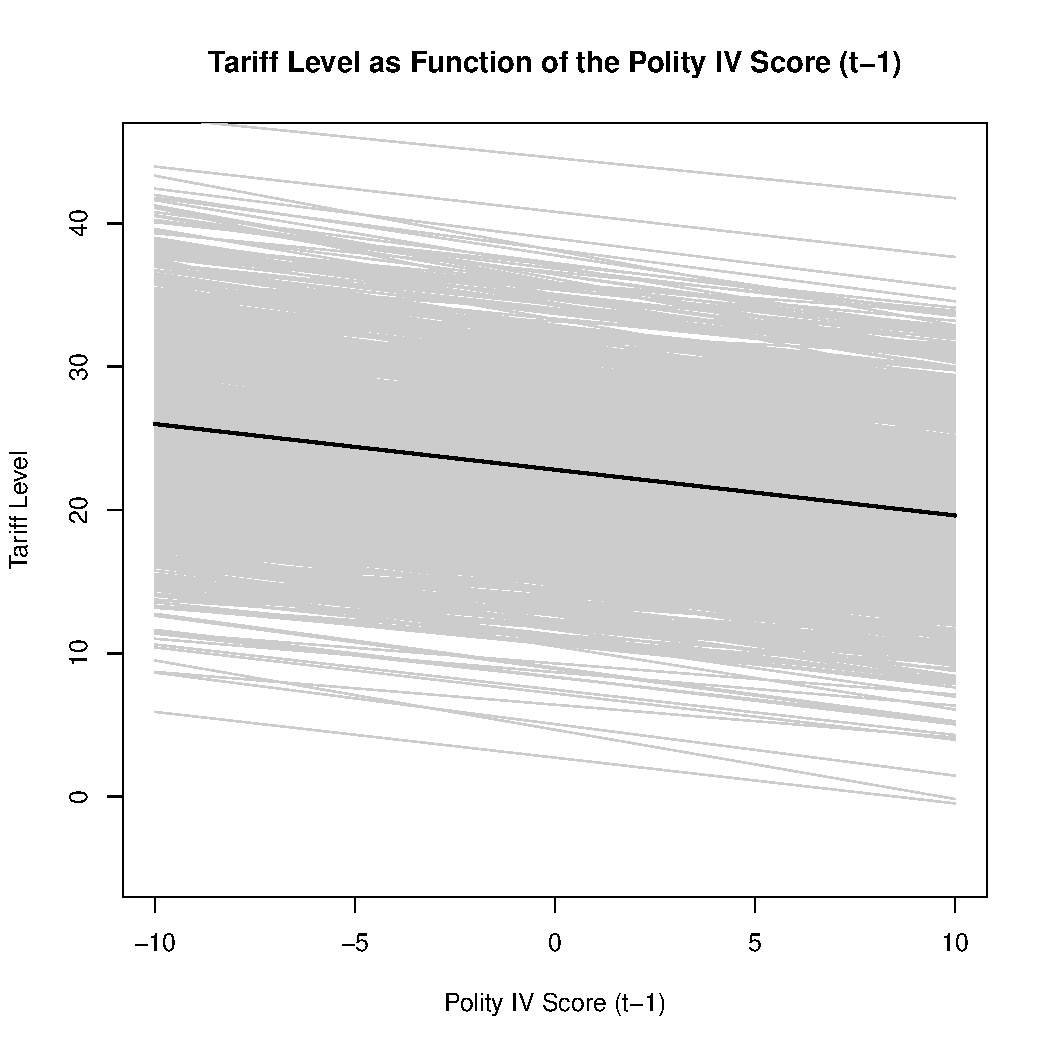
\includegraphics[width=\maxwidth]{figure/unnamed-chunk-7-1} 

\end{knitrout}



\subsection*{Problem 4}

\begin{knitrout}
\definecolor{shadecolor}{rgb}{0.969, 0.969, 0.969}\color{fgcolor}\begin{kframe}
\begin{alltt}
\hlkwd{quantile}\hlstd{(LDC}\hlopt{$}\hlstd{l1polity,} \hlkwc{probs} \hlstd{=} \hlkwd{c}\hlstd{(}\hlnum{0.25}\hlstd{,} \hlnum{0.75}\hlstd{),} \hlkwc{na.rm} \hlstd{= T)}
\end{alltt}
\begin{verbatim}
## 25% 75% 
##  -7   8
\end{verbatim}
\begin{alltt}
\hlkwd{quantile}\hlstd{(LDC}\hlopt{$}\hlstd{l1gdp_pc,} \hlkwc{probs} \hlstd{=} \hlkwd{c}\hlstd{(}\hlnum{0.25}\hlstd{,} \hlnum{0.75}\hlstd{),} \hlkwc{na.rm} \hlstd{= T)}
\end{alltt}
\begin{verbatim}
##       25%       75% 
##  458.8198 3225.3915
\end{verbatim}
\begin{alltt}
\hlkwd{quantile}\hlstd{(LDC}\hlopt{$}\hlstd{l1fdi,} \hlkwc{probs} \hlstd{=} \hlkwd{c}\hlstd{(}\hlnum{0.25}\hlstd{,} \hlnum{0.75}\hlstd{),} \hlkwc{na.rm} \hlstd{= T)}
\end{alltt}
\begin{verbatim}
##       25%       75% 
## 0.2185015 1.8839107
\end{verbatim}
\begin{alltt}
\hlcom{# Polity IV Score}

\hlstd{d.l1polity} \hlkwb{<-} \hlkwd{array}\hlstd{(}\hlnum{NA}\hlstd{,} \hlkwd{c}\hlstd{(}\hlnum{1000}\hlstd{,} \hlkwd{length}\hlstd{(LDC}\hlopt{$}\hlstd{newtar)))}
\hlstd{m.l1polity} \hlkwb{<-} \hlkwd{array}\hlstd{(}\hlnum{NA}\hlstd{,} \hlnum{1000}\hlstd{)}

\hlkwa{for} \hlstd{(i} \hlkwa{in} \hlnum{1}\hlopt{:}\hlnum{1000}\hlstd{) \{}
    \hlstd{d.l1polity[i, ]} \hlkwb{<-} \hlstd{(}\hlkwd{coef}\hlstd{(model.sims)[i,} \hlnum{1}\hlstd{]} \hlopt{+} \hlkwd{coef}\hlstd{(model.sims)[i,} \hlnum{2}\hlstd{]} \hlopt{*} \hlnum{8} \hlopt{+}
        \hlkwd{coef}\hlstd{(model.sims)[i,} \hlnum{3}\hlstd{]} \hlopt{*} \hlstd{LDC}\hlopt{$}\hlstd{l1signed} \hlopt{+} \hlkwd{coef}\hlstd{(model.sims)[i,} \hlnum{4}\hlstd{]} \hlopt{*} \hlstd{LDC}\hlopt{$}\hlstd{l1office} \hlopt{+}
        \hlkwd{coef}\hlstd{(model.sims)[i,} \hlnum{5}\hlstd{]} \hlopt{*} \hlstd{LDC}\hlopt{$}\hlstd{l1gdp_pc} \hlopt{+} \hlkwd{coef}\hlstd{(model.sims)[i,} \hlnum{6}\hlstd{]} \hlopt{*} \hlstd{LDC}\hlopt{$}\hlstd{l1lnpop} \hlopt{+}
        \hlkwd{coef}\hlstd{(model.sims)[i,} \hlnum{7}\hlstd{]} \hlopt{*} \hlstd{LDC}\hlopt{$}\hlstd{l1ecris2} \hlopt{+} \hlkwd{coef}\hlstd{(model.sims)[i,} \hlnum{8}\hlstd{]} \hlopt{*} \hlstd{LDC}\hlopt{$}\hlstd{l1bpc1)} \hlopt{-}
        \hlstd{(}\hlkwd{coef}\hlstd{(model.sims)[i,} \hlnum{1}\hlstd{]} \hlopt{+} \hlkwd{coef}\hlstd{(model.sims)[i,} \hlnum{2}\hlstd{]} \hlopt{* -}\hlnum{7} \hlopt{+} \hlkwd{coef}\hlstd{(model.sims)[i,}
            \hlnum{3}\hlstd{]} \hlopt{*} \hlstd{LDC}\hlopt{$}\hlstd{l1signed} \hlopt{+} \hlkwd{coef}\hlstd{(model.sims)[i,} \hlnum{4}\hlstd{]} \hlopt{*} \hlstd{LDC}\hlopt{$}\hlstd{l1office} \hlopt{+} \hlkwd{coef}\hlstd{(model.sims)[i,}
            \hlnum{5}\hlstd{]} \hlopt{*} \hlstd{LDC}\hlopt{$}\hlstd{l1gdp_pc} \hlopt{+} \hlkwd{coef}\hlstd{(model.sims)[i,} \hlnum{6}\hlstd{]} \hlopt{*} \hlstd{LDC}\hlopt{$}\hlstd{l1lnpop} \hlopt{+} \hlkwd{coef}\hlstd{(model.sims)[i,}
            \hlnum{7}\hlstd{]} \hlopt{*} \hlstd{LDC}\hlopt{$}\hlstd{l1ecris2} \hlopt{+} \hlkwd{coef}\hlstd{(model.sims)[i,} \hlnum{8}\hlstd{]} \hlopt{*} \hlstd{LDC}\hlopt{$}\hlstd{l1bpc1)}
    \hlstd{m.l1polity[i]} \hlkwb{<-} \hlkwd{mean}\hlstd{(d.l1polity[i, ])}
\hlstd{\}}

\hlkwd{mean}\hlstd{(m.l1polity)}
\end{alltt}
\begin{verbatim}
## [1] -4.791132
\end{verbatim}
\begin{alltt}
\hlkwd{sd}\hlstd{(m.l1polity)}
\end{alltt}
\begin{verbatim}
## [1] 1.337032
\end{verbatim}
\begin{alltt}
\hlkwd{quantile}\hlstd{(m.l1polity,} \hlkwc{probs} \hlstd{=} \hlkwd{c}\hlstd{(}\hlnum{0.025}\hlstd{,} \hlnum{0.16}\hlstd{,} \hlnum{0.84}\hlstd{,} \hlnum{0.975}\hlstd{))}
\end{alltt}
\begin{verbatim}
##      2.5%       16%       84%     97.5% 
## -7.380059 -6.074565 -3.481395 -2.195121
\end{verbatim}
\begin{alltt}
\hlcom{# GDP per Capita}

\hlstd{d.l1gdp_pc} \hlkwb{<-} \hlkwd{array}\hlstd{(}\hlnum{NA}\hlstd{,} \hlkwd{c}\hlstd{(}\hlnum{1000}\hlstd{,} \hlkwd{length}\hlstd{(LDC}\hlopt{$}\hlstd{newtar)))}
\hlstd{m.l1gdp_pc} \hlkwb{<-} \hlkwd{array}\hlstd{(}\hlnum{NA}\hlstd{,} \hlnum{1000}\hlstd{)}

\hlkwa{for} \hlstd{(i} \hlkwa{in} \hlnum{1}\hlopt{:}\hlnum{1000}\hlstd{) \{}
    \hlstd{d.l1gdp_pc[i, ]} \hlkwb{<-} \hlstd{(}\hlkwd{coef}\hlstd{(model.sims)[i,} \hlnum{1}\hlstd{]} \hlopt{+} \hlkwd{coef}\hlstd{(model.sims)[i,} \hlnum{2}\hlstd{]} \hlopt{*} \hlstd{LDC}\hlopt{$}\hlstd{l1polity} \hlopt{+}
        \hlkwd{coef}\hlstd{(model.sims)[i,} \hlnum{3}\hlstd{]} \hlopt{*} \hlstd{LDC}\hlopt{$}\hlstd{l1signed} \hlopt{+} \hlkwd{coef}\hlstd{(model.sims)[i,} \hlnum{4}\hlstd{]} \hlopt{*} \hlstd{LDC}\hlopt{$}\hlstd{l1office} \hlopt{+}
        \hlkwd{coef}\hlstd{(model.sims)[i,} \hlnum{5}\hlstd{]} \hlopt{*} \hlnum{3225.3915} \hlopt{+} \hlkwd{coef}\hlstd{(model.sims)[i,} \hlnum{6}\hlstd{]} \hlopt{*} \hlstd{LDC}\hlopt{$}\hlstd{l1lnpop} \hlopt{+}
        \hlkwd{coef}\hlstd{(model.sims)[i,} \hlnum{7}\hlstd{]} \hlopt{*} \hlstd{LDC}\hlopt{$}\hlstd{l1ecris2} \hlopt{+} \hlkwd{coef}\hlstd{(model.sims)[i,} \hlnum{8}\hlstd{]} \hlopt{*} \hlstd{LDC}\hlopt{$}\hlstd{l1bpc1)} \hlopt{-}
        \hlstd{(}\hlkwd{coef}\hlstd{(model.sims)[i,} \hlnum{1}\hlstd{]} \hlopt{+} \hlkwd{coef}\hlstd{(model.sims)[i,} \hlnum{2}\hlstd{]} \hlopt{*} \hlstd{LDC}\hlopt{$}\hlstd{l1polity} \hlopt{+} \hlkwd{coef}\hlstd{(model.sims)[i,}
            \hlnum{3}\hlstd{]} \hlopt{*} \hlstd{LDC}\hlopt{$}\hlstd{l1signed} \hlopt{+} \hlkwd{coef}\hlstd{(model.sims)[i,} \hlnum{4}\hlstd{]} \hlopt{*} \hlstd{LDC}\hlopt{$}\hlstd{l1office} \hlopt{+} \hlkwd{coef}\hlstd{(model.sims)[i,}
            \hlnum{5}\hlstd{]} \hlopt{*} \hlnum{458.8198} \hlopt{+} \hlkwd{coef}\hlstd{(model.sims)[i,} \hlnum{6}\hlstd{]} \hlopt{*} \hlstd{LDC}\hlopt{$}\hlstd{l1lnpop} \hlopt{+} \hlkwd{coef}\hlstd{(model.sims)[i,}
            \hlnum{7}\hlstd{]} \hlopt{*} \hlstd{LDC}\hlopt{$}\hlstd{l1ecris2} \hlopt{+} \hlkwd{coef}\hlstd{(model.sims)[i,} \hlnum{8}\hlstd{]} \hlopt{*} \hlstd{LDC}\hlopt{$}\hlstd{l1bpc1)}
    \hlstd{m.l1gdp_pc[i]} \hlkwb{<-} \hlkwd{mean}\hlstd{(d.l1gdp_pc[i, ])}
\hlstd{\}}

\hlkwd{mean}\hlstd{(m.l1gdp_pc)}
\end{alltt}
\begin{verbatim}
## [1] -3.427087
\end{verbatim}
\begin{alltt}
\hlkwd{sd}\hlstd{(m.l1gdp_pc)}
\end{alltt}
\begin{verbatim}
## [1] 0.4298
\end{verbatim}
\begin{alltt}
\hlkwd{quantile}\hlstd{(m.l1gdp_pc,} \hlkwc{probs} \hlstd{=} \hlkwd{c}\hlstd{(}\hlnum{0.025}\hlstd{,} \hlnum{0.16}\hlstd{,} \hlnum{0.84}\hlstd{,} \hlnum{0.975}\hlstd{))}
\end{alltt}
\begin{verbatim}
##      2.5%       16%       84%     97.5% 
## -4.282437 -3.828239 -3.015397 -2.558968
\end{verbatim}
\begin{alltt}
\hlcom{# Plot}

\hlkwd{plot}\hlstd{(}\hlnum{1}\hlopt{:}\hlnum{2}\hlstd{,} \hlkwd{c}\hlstd{(}\hlkwd{mean}\hlstd{(m.l1polity),} \hlkwd{mean}\hlstd{(m.l1gdp_pc)),} \hlkwc{type} \hlstd{=} \hlstr{"p"}\hlstd{,} \hlkwc{ylim} \hlstd{=} \hlkwd{c}\hlstd{(}\hlopt{-}\hlnum{8}\hlstd{,} \hlnum{0}\hlstd{),}
    \hlkwc{xlim} \hlstd{=} \hlkwd{c}\hlstd{(}\hlnum{0}\hlstd{,} \hlnum{2}\hlstd{),} \hlkwc{xlab} \hlstd{=} \hlstr{""}\hlstd{,} \hlkwc{main} \hlstd{=} \hlstr{"Polity IV Score, GDP per Capita, and Tariff Levels"}\hlstd{,}
    \hlkwc{ylab} \hlstd{=} \hlstr{"Average predictive comparison (25th to 75th perc.)"}\hlstd{,} \hlkwc{asp} \hlstd{=} \hlnum{1.5}\hlstd{,}
    \hlkwc{axes} \hlstd{=} \hlnum{FALSE}\hlstd{)}
\hlkwd{axis}\hlstd{(}\hlnum{1}\hlstd{,} \hlkwc{at} \hlstd{=} \hlkwd{c}\hlstd{(}\hlnum{1}\hlstd{,} \hlnum{2}\hlstd{),} \hlkwc{labels} \hlstd{=} \hlkwd{c}\hlstd{(}\hlstr{"Polity"}\hlstd{,} \hlstr{"GDP"}\hlstd{))}
\hlkwd{axis}\hlstd{(}\hlnum{2}\hlstd{,} \hlkwc{at} \hlstd{=} \hlkwd{seq}\hlstd{(}\hlopt{-}\hlnum{8}\hlstd{,} \hlnum{0}\hlstd{,} \hlkwc{by} \hlstd{=} \hlnum{1}\hlstd{))}
\hlkwd{abline}\hlstd{(}\hlkwc{h} \hlstd{=} \hlnum{0}\hlstd{,} \hlkwc{lty} \hlstd{=} \hlnum{2}\hlstd{)}
\hlkwd{segments}\hlstd{(}\hlnum{1}\hlstd{,} \hlkwd{quantile}\hlstd{(m.l1polity,} \hlkwc{probs} \hlstd{=} \hlkwd{c}\hlstd{(}\hlnum{0.025}\hlstd{)),} \hlnum{1}\hlstd{,} \hlkwd{quantile}\hlstd{(m.l1polity,}
    \hlkwc{probs} \hlstd{=} \hlkwd{c}\hlstd{(}\hlnum{0.975}\hlstd{)))}
\hlkwd{segments}\hlstd{(}\hlnum{2}\hlstd{,} \hlkwd{quantile}\hlstd{(m.l1gdp_pc,} \hlkwc{probs} \hlstd{=} \hlkwd{c}\hlstd{(}\hlnum{0.025}\hlstd{)),} \hlnum{2}\hlstd{,} \hlkwd{quantile}\hlstd{(m.l1gdp_pc,}
    \hlkwc{probs} \hlstd{=} \hlkwd{c}\hlstd{(}\hlnum{0.975}\hlstd{)))}
\end{alltt}
\end{kframe}
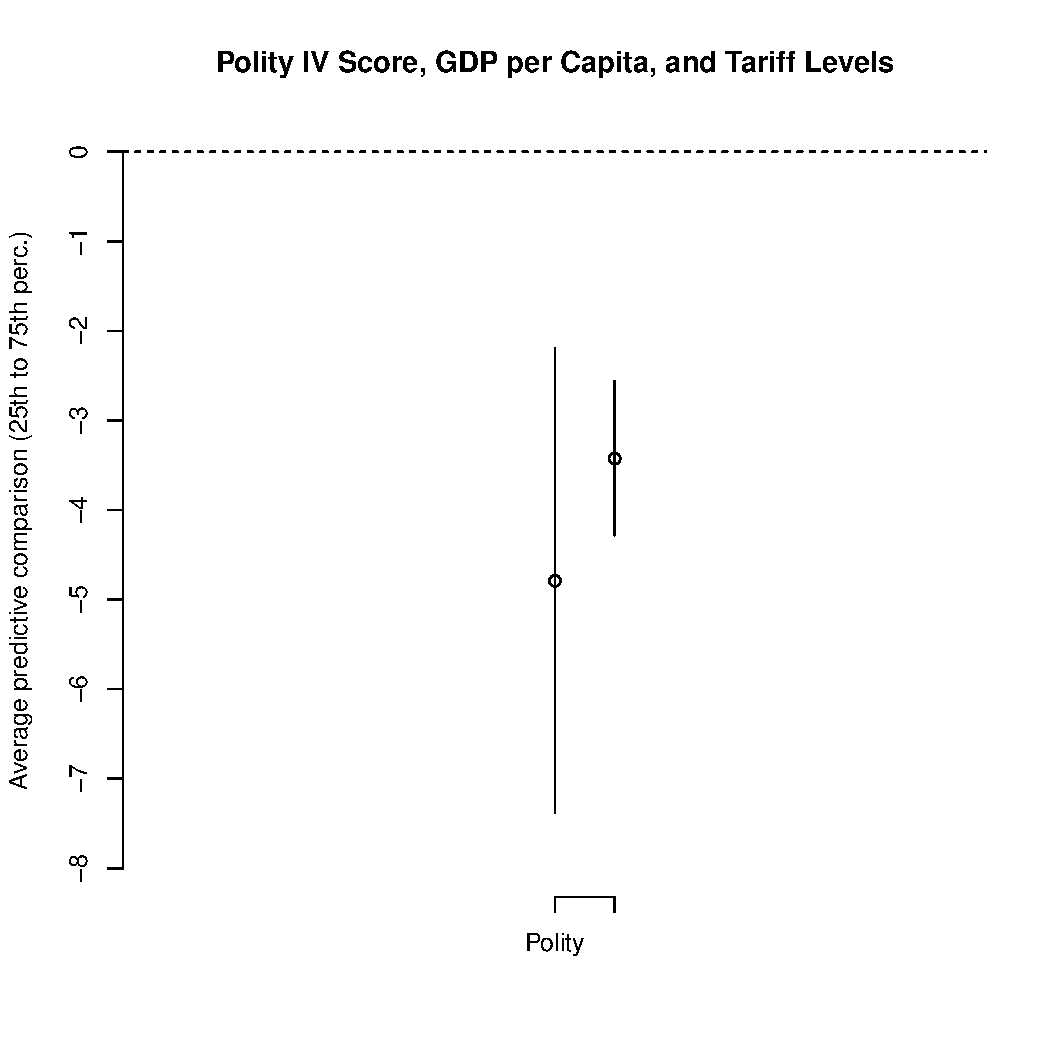
\includegraphics[width=\maxwidth]{figure/unnamed-chunk-8-1} 

\end{knitrout}

Interpretation: although the Polity IV Score appears to have the larger average substantive effect (when looking at changes from the 25th to the 75th percentile value), there is also greater uncertainty about its impact. The mean effect of GDP per capita changes (for the same percentile values) is smaller but uncertainty about the effect is smaller as well. Considering both the means and the confidence intervals, we cannot make any definitive statements about which variable has the greater substantive impact, but the Polity-IV score is likely to have a larger one considering these results.

Note: It is fine to say that there is no significant visible difference if you are grading someone's homework and the person has arrived at this conclusion.


\end{document}
